\chapter{AI 赋能专题}
\definecolor{researchBlue}{HTML}{25465D}
\definecolor{researchTeal}{HTML}{287B78}
\definecolor{researchBronze}{HTML}{B67E33}
\definecolor{researchInk}{HTML}{243348}

开发时，我们请 AI 帮忙整理需求、起草代码和补全测试输入，草稿交回组员逐项复核。系统交付之后，顾客也能从点餐页进入问答、商品推荐、图片识菜和语音点菜。前一项查草稿里的业务规则，后一项查顾客实际看到的商品和订单。

\section{AI 赋能全景架构}

图~\ref{fig:ai-dual-arch} 左侧从 SRS 用例走到人工审查和回归测试。右侧从顾客发出请求开始，系统根据输入选择本地问答、菜单筛选或外部模型，调用出错时再按已有规则返回。

\begin{figure}[!htbp]
  \centering
  \resizebox{.96\linewidth}{!}{\begin{tikzpicture}[x=1pt,y=1pt,
    title/.style={anchor=west,inner sep=0pt,font=\small\bfseries},
    workflow step/.style={inner sep=0pt,anchor=west,align=left,
      font=\linespread{1}\fontsize{9.6bp}{12bp}\selectfont,text=black!88}]
  \foreach \start/\stop/\tone/\name in {
    0/178/researchBlue/{研发过程中的 AI 协作},
    200/422/researchTeal/{点餐流程中的多模态 AI}} {
    \node[title,text=\tone] at (\start,0) {\name};
    \draw[\tone,line width=.84pt] (\start,-12) -- (\stop,-12);
    \foreach \from/\to in {-33/-69,-69/-105,-105/-141} {
      \draw[\tone,line width=.62pt,-{Stealth[length=3.3pt,width=3.1pt]}]
        (\start+4,\from-4) -- (\start+4,\to+5.5);
    }
    \foreach \row in {-33,-69,-105,-141}
      \fill[\tone] (\start+4,\row) circle[radius=2.9pt];
  }
  \node[workflow step] at (16,-33) {补全 SRS 用例并核查差异};
  \node[workflow step] at (16,-69) {SQL 幂等迁移与接口契约核对};
  \node[workflow step] at (16,-105) {生成代码样板与 TDD 边界用例};
  \node[workflow step] at (16,-141) {人工走查与 575 项自动化测试};
  \node[workflow step] at (216,-33) {文字对话与规则问答\\{\textcolor{black!63}{DeepSeek / 本地帮助}}};
  \node[workflow step] at (216,-69) {条件智能筛选\\{\textcolor{black!63}{真实菜单库存 + 一键加购}}};
  \node[workflow step] at (216,-105) {多模态识别\\{\textcolor{black!63}{DashScope 图片识菜 / 语音草稿}}};
  \node[workflow step] at (216,-141) {身份注入、事务外调用、熔断与降级};
\end{tikzpicture}
}
  \caption{项目研发过程与系统运行时双维 AI 赋能全景架构图}\label{fig:ai-dual-arch}
\end{figure}

\section{研发过程全流程 AI 赋能实践}

\subsection{各工程阶段的 AI 协同应用}

整理 SRS 时，人容易顺着成功流程往下写。我们让 AI 帮忙找没交代的分支，比如店铺休息后还能不能加购、库存不足时哪些写入要回滚。产品负责人拿着这些问题去查页面与代码。碰到订单阶段在文档里有两个叫法，就先核准状态值和各端能做的动作，再统一用词。课上讲的需求核查，在这里帮我们把一个模糊的状态词改成了可以逐端检查的条件。

给快照、备注和坐标加列时，我们让 AI 参照已有的 SQL 起草 \code{003}、\code{005} 和 \code{006} 的修改模板。列能否为空、以前的订单能从哪里读数据，留给组员查旧记录后决定。DTO 校验、MyBatis 映射和 CSS 主题变量也可以从草稿开始。合入之前，负责同学回到已有接口和数据，核对字段、权限来源以及旧版本留下的记录。

\subsection{人机协同工作闭环}

给 AI 提任务时，我们会先带上项目现有的 DTO、表结构和业务条件，图~\ref{fig:ai-collab-loop} 左边就是这一步。拿到草稿以后，组员检查身份来源、更新条件、空值和事务的起止，约定应当看到的结果，再运行 \code{./mvnw test} 和 \code{npm test}。管理员检索这类时序问题，AI 能提示几处可疑调用，哪次请求回来得晚，仍要靠浏览器里的复现和写好的用例来确认。

\subsection{人工核查怎样落到代码}

评审 AI 对话控制器时，我们发现 DTO 草稿允许请求写入 \mbox{\code{userId}}。于是将 \mbox{\code{AiChatRequestDTO.userId}} 设为 \mbox{\code{READ_ONLY}}，改由后端从认证上下文取得当前用户。我们也把模型请求移到事务之外，收到回复再写入对话。等待网络响应时，数据库连接仍可供其他请求使用。

我们评审测试草稿时也会追问它最后比较了哪个值。结算接口响应成功以后，还要查清用的是哪一份价格。\code{OrderPricingTrustBoundaryTest} 对照服务端算出的应收金额，检查请求多传的价格字段是否改变结果。图片或语音服务缺少密钥时，后端统一返回 \code{503 FEATURE_UNAVAILABLE}，前端再给出具体提示。这些结果写成断言以后，每次回归都能再查一遍。

\begin{figure}[!htbp]
  \centering
  \resizebox{0.98\linewidth}{!}{%
\begin{tikzpicture}[
    x=1pt,y=1pt,
    review box/.style={rectangle,rounded corners=2.5pt,align=center,
      minimum height=40pt,minimum width=96pt,inner xsep=2pt,inner ysep=3pt,
      draw=researchBlue!66,fill=researchBlue!7,text=researchInk,
      line width=.55pt,font=\fontsize{9.3bp}{13bp}\selectfont},
    arr/.style={-{Stealth[length=4pt,width=3.4pt]},line width=.66pt,draw=researchInk!80}
  ]
    \node[review box] (s1) at (48,0) {\textbf{1. 约束输入}\\锁定 DTO/表/红线};
    \node[review box] (s2) at (155.5,0) {\textbf{2. 辅助产出}\\样板/SQL/用例草稿};
    \node[review box,draw=researchBronze!80,fill=researchBronze!9] (s3) at (263,0)
      {\textbf{3. 人工审计}\\查鉴权/事务/断言};
    \node[review box,draw=researchTeal!75,fill=researchTeal!8] (s4) at (370.5,0)
      {\textbf{4. 门禁验证}\\575 项回归与 PR 合入};
    \foreach \srcnode/\dstnode in {s1/s2,s2/s3,s3/s4}
      \draw[arr] (\srcnode.east) -- (\dstnode.west);
    \draw[arr,densely dashed,draw=researchBronze] (s3.south) -- (263,-37) --
      node[midway,below=2pt,text=researchBronze!80!black,font=\fontsize{8.7bp}{10bp}\selectfont]
        {发现隐式漂移则打回重写} (48,-37) -- (s1.south);
  \end{tikzpicture}
}
  \caption{研发过程四步人机协同审计闭环流程图}\label{fig:ai-collab-loop}
\end{figure}



\section{系统运行时 AI 业务能力设计与落地}

\subsection{多模态 AI 服务矩阵}

顾客从 \code{/ai-chat} 和相应子页面进入助手。想问规则可以直接输入文字，想找菜就给预算和菜名，也可以上传图片或音频。点餐页提供文字对话、规则推荐、图片识菜和语音草稿四个入口，接口、模型及服务不可用时的处理见附录表~\ref{tab:runtime-ai-matrix}。

\subsection{意图分流、安全隔离与熔断降级设计}

顾客问退款规则时，已有的说明就能回答。图片识菜和语音转写则要联系外部服务。图~\ref{fig:ai-guardrails} 把本地与外部调用分别画出来。两条路径都要确认谁在提问、回复可用哪些数据，以及结果返回后要写入什么。

\begin{reportpoints}
  \item 候选菜品来自当前在售且有足够库存的菜单。加购由顾客在卡片上确认，金额仍由购物车和结算接口计算。
  \item 用户 ID 取自认证上下文。订单查询限定在当前用户，待查询的业务内容按数据处理，日志隐藏对话正文。
  \item 模型请求在数据库事务外完成，收到响应后再用短事务写入 \code{ai_chat_history}。
  \item 外部调用受总超时、熔断和重试上限管理。重试上限默认为 3 次。缺少密钥或模型调用失败时，可使用本地帮助与推荐。
\end{reportpoints}

\begin{figure}[!htbp]
  \centering
  \resizebox{0.98\linewidth}{!}{%
\begin{tikzpicture}[
    x=1pt,y=1pt,
    blk/.style={rectangle,rounded corners=2pt,align=center,minimum width=76pt,
      minimum height=39pt,inner xsep=2pt,inner ysep=3pt,line width=.55pt,
      draw=researchBlue!66,fill=researchBlue!7,text=researchInk,
      font=\fontsize{8.6bp}{11.2bp}\selectfont},
    dec/.style={diamond,aspect=1.27,align=center,inner sep=1pt,line width=.55pt,
      draw=researchBronze!86,fill=researchBronze!9,text=researchInk,
      font=\fontsize{8.4bp}{11bp}\selectfont},
    branch/.style={blk,minimum width=112pt,minimum height=38pt},
    arr/.style={-{Stealth[length=3.6pt,width=3.2pt]},line width=.62pt,draw=researchInk!84},
    signal/.style={text=researchInk,fill=white,inner sep=1.5pt,
      font=\fontsize{8.3bp}{10bp}\selectfont}
  ]
    \node[blk] (in) at (38,0) {\textbf{用户多模态输入}\\文本 / 图片 / 语音};
    \node[blk] (ctx) at (127,0) {\textbf{JWT 身份注入}\\剥离伪造 userId};
    \node[dec] (intent) at (215,0) {意图分流\\与密钥检查};
    \node[branch,draw=researchTeal!75,fill=researchTeal!8] (local) at (309,38)
      {\textbf{本地规则 / 订单查询}\\查库真实菜单与本人订单};
    \node[branch,draw=researchBronze!78,fill=researchBronze!8] (ext) at (309,-38)
      {\textbf{脱事务外部调用}\\超时控制 + \texttt{AiCircuitBreaker}};
    \node[blk,draw=researchTeal!75,fill=researchTeal!8] (out) at (416,0)
      {\textbf{结构化候选输出}\\卡片一键加购\\/ 503 降级};

    \draw[arr] (in.east) -- (ctx.west);
    \draw[arr] (ctx.east) -- (intent.west);
    \draw[arr,draw=researchTeal] (intent.north) |- (local.west);
    \node[signal,above right] at (186,38) {本地意图/无Key};
    \draw[arr,draw=researchBronze] (intent.south) |- (ext.west);
    \node[signal,below right] at (186,-38) {外部增强意图};
    \draw[arr,draw=researchTeal] (local.east) -| (out.north);
    \draw[arr,draw=researchBronze] (ext.east) -| (out.south);
  \end{tikzpicture}
}
  \caption{运行时 AI 意图分流、脱事务外部调用与四重安全护栏流程图}\label{fig:ai-guardrails}
\end{figure}

顾客说“某个价格以内想吃什么”时，预算从表单或问题文本取出。推荐服务先用库存筛掉不能买的商品，再把起送差额、配送费和店铺满减算进去，估算最低结算金额。菜单卡片只是推荐结果，顾客点选以后，购物车再按当时的店铺和库存接受加购。

\subsection{从输入到推荐结果}

助手收到文字后，先确认登录用户及会话归属，再根据关键词处理。退款、会员一类疑问从本地规则找答案，提到订单与配送时转到订单对话，给了菜名或预算就从菜单筛。一般对话和订单对话经 \code{AiChatServiceImpl}，模型不可用时由本地分支接手。几种回复共用一个历史服务，重新打开相应会话时仍能读到之前的问答。

\code{AssistantIntegrationTest} 用商品数量、预算和库存来查推荐结果。同时，它也查两张表。推荐完成以后，应新增一条对话历史，购物车保持为空。顾客看完结果后自己决定加购，测试把这条分界固定下来了。相同套件还分别试了未登录访问和跨用户会话，后者在生成回复前就被拒绝。

\subsubsection{文字问答的调用与保存}

图~\ref{fig:ai-chat-history-sequence-uml} 展开 \code{AiChatServiceImpl.chat} 的调用。服务从当前登录会话取用户编号，再核对会话归属。配置了密钥时，服务先尝试让 DeepSeek 生成回复。若没有可用文本，便由本地规则生成答案。这时页面看到的来源也改为本地。

\begin{figure}[!htbp]
  \centering
  \begin{tikzpicture}[
  x=1pt,y=-1pt,
  line width=.46pt,
  annotate/.style={fill=white,align=center,inner sep=1.7pt},
  participant/.style={draw,fill=white,align=center,minimum height=27pt,inner sep=2pt,font=\bfseries},
  activation/.style={draw,fill=white},
  lifeline/.style={dash pattern=on 3pt off 2pt},
  call/.style={-{Stealth[length=4.7pt,width=4.4pt]}},
  reply/.style={dash pattern=on 3pt off 2pt,-{Straight Barb[length=4.4pt,width=4.4pt]}},
  every node/.style={font=\linespread{1}\fontsize{10bp}{11.4bp}\selectfont}
]
  \foreach \x in {27,91,157,236,307,378} {
    \draw[lifeline] (\x,27) -- (\x,304);
  }
  \node[participant,minimum width=49pt,anchor=north] at (27,0) {Web 客户端};
  \node[participant,minimum width=60pt,anchor=north] at (91,0) {\texttt{AiChat}\\\texttt{Controller}};
  \node[participant,minimum width=65pt,anchor=north] at (157,0) {\texttt{AiChatService}\\\texttt{Impl}};
  \node[participant,minimum width=64pt,anchor=north] at (236,0) {\texttt{DeepSeek}\\\texttt{ApiClient}};
  \node[participant,minimum width=63pt,anchor=north] at (307,0) {\texttt{LocalAi}\\\texttt{Responder}};
  \node[participant,minimum width=71pt,anchor=north] at (378,0) {\texttt{AiChatHistory}\\\texttt{Service}};

  \draw (104,109) rectangle (417,161);
  \draw (104,109) -- (135,109) -- (135,119) -- (130,124) -- (104,124);
  \node[font=\bfseries] at (119,116.5) {opt};
  \node[annotate,anchor=west] at (166,118) {[配置了非空白 API 密钥]};
  \draw (104,170) rectangle (417,222);
  \draw (104,170) -- (135,170) -- (135,180) -- (130,185) -- (104,185);
  \node[font=\bfseries] at (119,177.5) {opt};
  \node[annotate,anchor=west] at (166,179) {[\texttt{message == null}]};

  \draw[activation] (87.5,45) rectangle (94.5,294);
  \draw[activation] (153.5,64) rectangle (160.5,276);
  \draw[activation] (374.5,85) rectangle (381.5,100);
  \draw[activation] (232.5,138) rectangle (239.5,154);
  \draw[activation] (303.5,199) rectangle (310.5,214);
  \draw[activation] (374.5,242) rectangle (381.5,259);

  \draw[call] (27,45) -- node[annotate,above] {\texttt{POST /api/ai/chat}} (87.5,45);
  \draw[call] (94.5,64) -- node[annotate,above] {\texttt{chat(request)}} (153.5,64);
  \draw[call] (160.5,85) -- node[annotate,above] {\texttt{requireWritableSession(sessionId)}} (374.5,85);
  \draw[reply] (374.5,100) -- node[annotate,above] {会话写权限校验通过} (160.5,100);

  \draw[call] (160.5,138) -- node[annotate,above] {同步请求模型} (232.5,138);
  \draw[reply] (232.5,154) -- node[annotate,above] {响应或异常} (160.5,154);
  \node[annotate,anchor=west] at (248,140) {取第一候选的非空白正文};
  \node[annotate,anchor=west] at (248,153) {运行时异常时回复仍为空};

  \draw[call] (160.5,199) -- node[annotate,above] {\texttt{reply(request)}} (303.5,199);
  \draw[reply] (303.5,214) -- node[annotate,above] {本地规则回复} (160.5,214);

  \draw[call] (160.5,242) -- node[annotate,above] {\texttt{save(request, response)}} (374.5,242);
  \node[annotate,anchor=east] (saveNote) at (368,249.5)
    {\texttt{@Transactional} 内重校会话并写入记录};
  \draw[densely dotted] (saveNote.east) -- (374.5,249.5);
  \draw[reply] (374.5,259) -- node[annotate,below] {保存正常完成} (160.5,259);

  \draw[reply] (153.5,276) -- node[annotate,above] {回复对象} (94.5,276);
  \draw[reply] (87.5,294) -- node[annotate,above] {成功响应} (27,294);
\end{tikzpicture}

  \caption{文字问答生成、回退与历史保存（UML 时序图）}\label{fig:ai-chat-history-sequence-uml}
\end{figure}

得到回复后，历史服务在单独的事务内重查会话归属，再写入本轮问答。写入完成后控制器才返回成功。联调时可以把回复里标明的来源与同一会话的历史记录对照，分别核对是谁生成了这条回复，以及页面下次打开时能否读回。

\subsection{模型适配与异常回归}

图片里识别出的菜名先拿到平台菜单里匹配，遇到重复的候选就合并。语音转出来的文字则先整理成草稿，留给用户核对菜名和份数。我们在单元测试里给定识别结果。一例返回两份牛肉面，再查候选能不能对上。浏览器里的录音还得考虑人什么时候关闭抽屉。打开后马上关掉，权限回调即使晚到，音轨也要及时释放。

为了单独检查外部调用要等多久，\code{DeepSeekDeadlineTest} 在本机起了一个模拟服务，让它等 3 秒才响应。客户端的总超时为 1 秒，重试上限为 3 次。测试看到调用在总限时内失败，模拟端只收到 1 次正式请求。它把超时后是否继续重试查清了，浏览器上的提示则用来确认用户遇到的是哪种情况。模型和端点配置见表~\ref{tab:runtime-ai-matrix}。

\Needspace{6\baselineskip}
\subsection{演示环境验证}

我们走查的演示环境没有配 DeepSeek 和 DashScope 密钥。打开问答客服能看到欢迎页与快捷问题，切到智能筛选后，输入“鸡腿饭”和 30 元预算，页面从演示库里找出了在售商品。图~\ref{fig:ai-qa-recommend} 记录了本地筛选返回的菜品和加购入口。

\Needspace{.58\textheight}
问答页把提问、历史和快捷入口放在一起。从“20 元内吃什么”这类快捷问题开始，顾客还可以补充要求。智能筛选则用两个表单项保留关键词和预算，拿到结果后仍能看到之前填了什么。图中照烧鸡腿饭是 18.80 元，脆皮鸡腿堡是 19.90 元，与演示菜单上的同名商品一致。每张卡片右侧都能点选加购。

\begin{figure}[H]
  \centering
  \begin{minipage}[t]{.48\linewidth}
    \vspace{0pt}\centering
    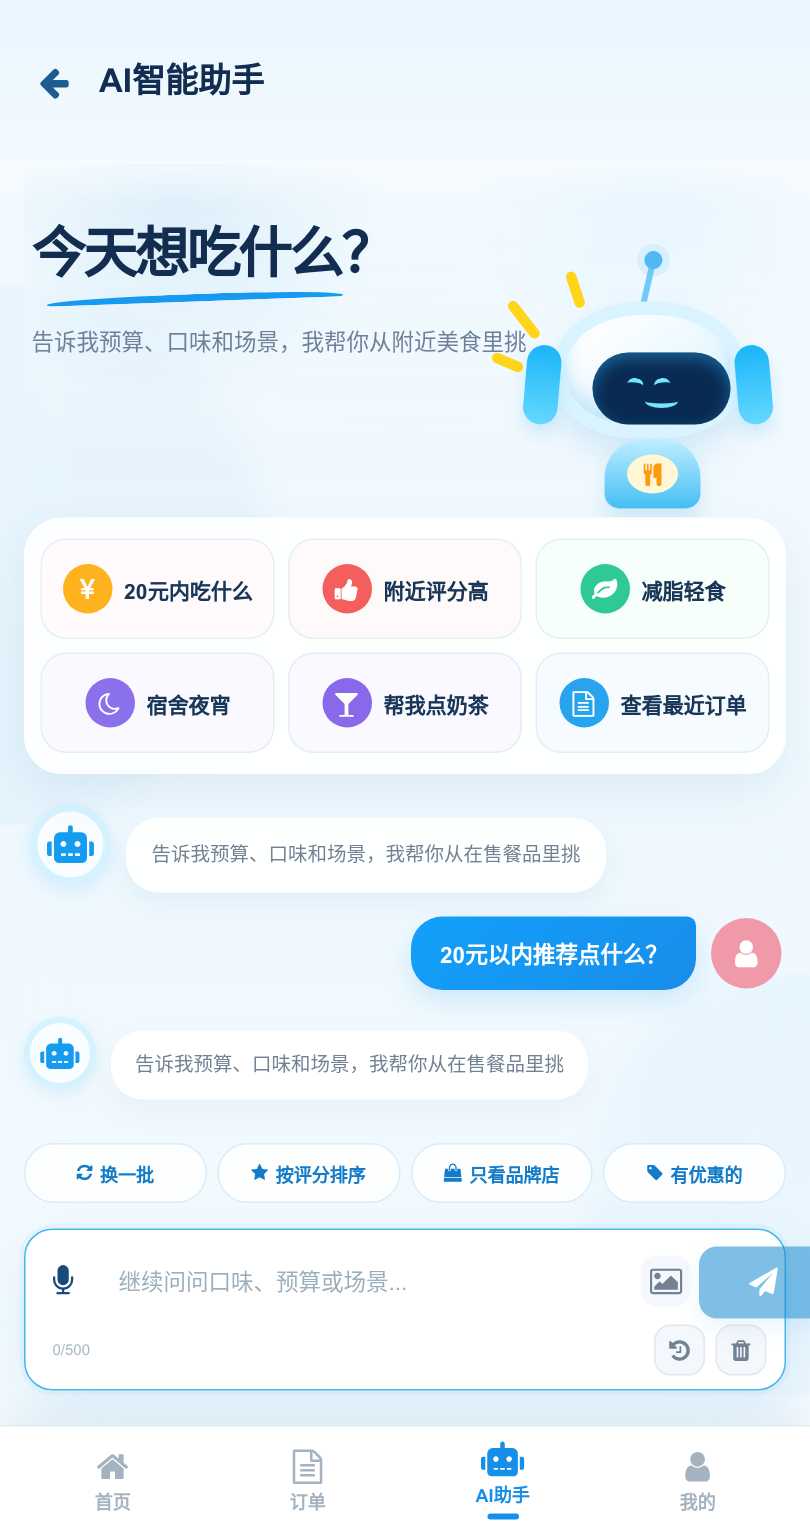
\includegraphics[width=\linewidth,height=.44\textheight,keepaspectratio]{figures/screenshots/ui-ai-chat-qa.png}\par\smallskip
    {\small （a）AI 问答客服入口与快捷提问气泡（\code{/ai-chat}）}
  \end{minipage}\hfill
  \begin{minipage}[t]{.48\linewidth}
    \vspace{0pt}\centering
    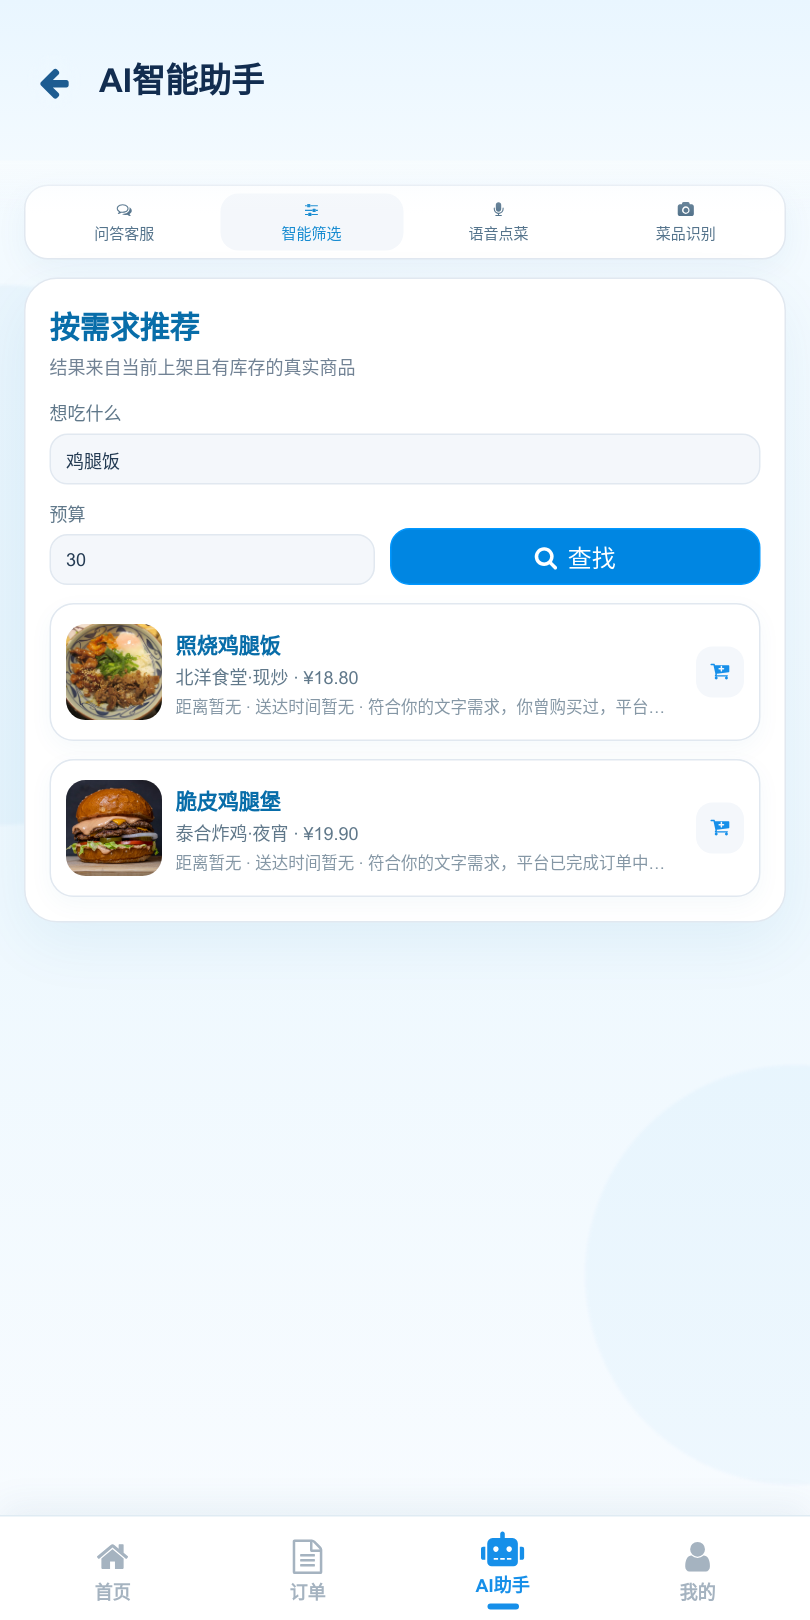
\includegraphics[width=\linewidth,height=.44\textheight,keepaspectratio]{figures/screenshots/ui-ai-assistant.png}\par\smallskip
    {\small （b）智能筛选本地规则推荐结果（真实在售菜单）}
  \end{minipage}
  \caption{AI 智能客服与本地规则推荐界面实景截图（未调用外部大模型）}\label{fig:ai-qa-recommend}\label{fig:ai-runtime-placeholder}
\end{figure}

卡片显示店铺名与商品单价，预算筛选用的却是算上配送和优惠后的最低结算金额。复查时，我们从卡片回到具体店铺和菜品，再对照原来的推荐条件。点了加购之后，还能用购物车里的商品和数量核对下一步。

\clearpage
图~\ref{fig:ai-voice-media} 是语音与图片服务未配置时的页面。我们分别查了录音、文件选择和图片上传入口。这些入口也可以沿用到配置模型后的验收，用于核对浏览器权限和实际识别结果。

页面打开时先请求 \code{/api/v1/assistant/capabilities}。图左的录音和选择音频按钮下方提示语音模型未配置，图右也因缺少识菜模型关闭了图片入口。如果能读到能力状态，就把缺少的那项服务写清楚。如果能力请求本身失败，页面会让用户检查连接，并留出重试入口。

\begin{figure}[H]
  \centering
  \begin{minipage}[t]{.48\linewidth}
    \vspace{0pt}\centering
    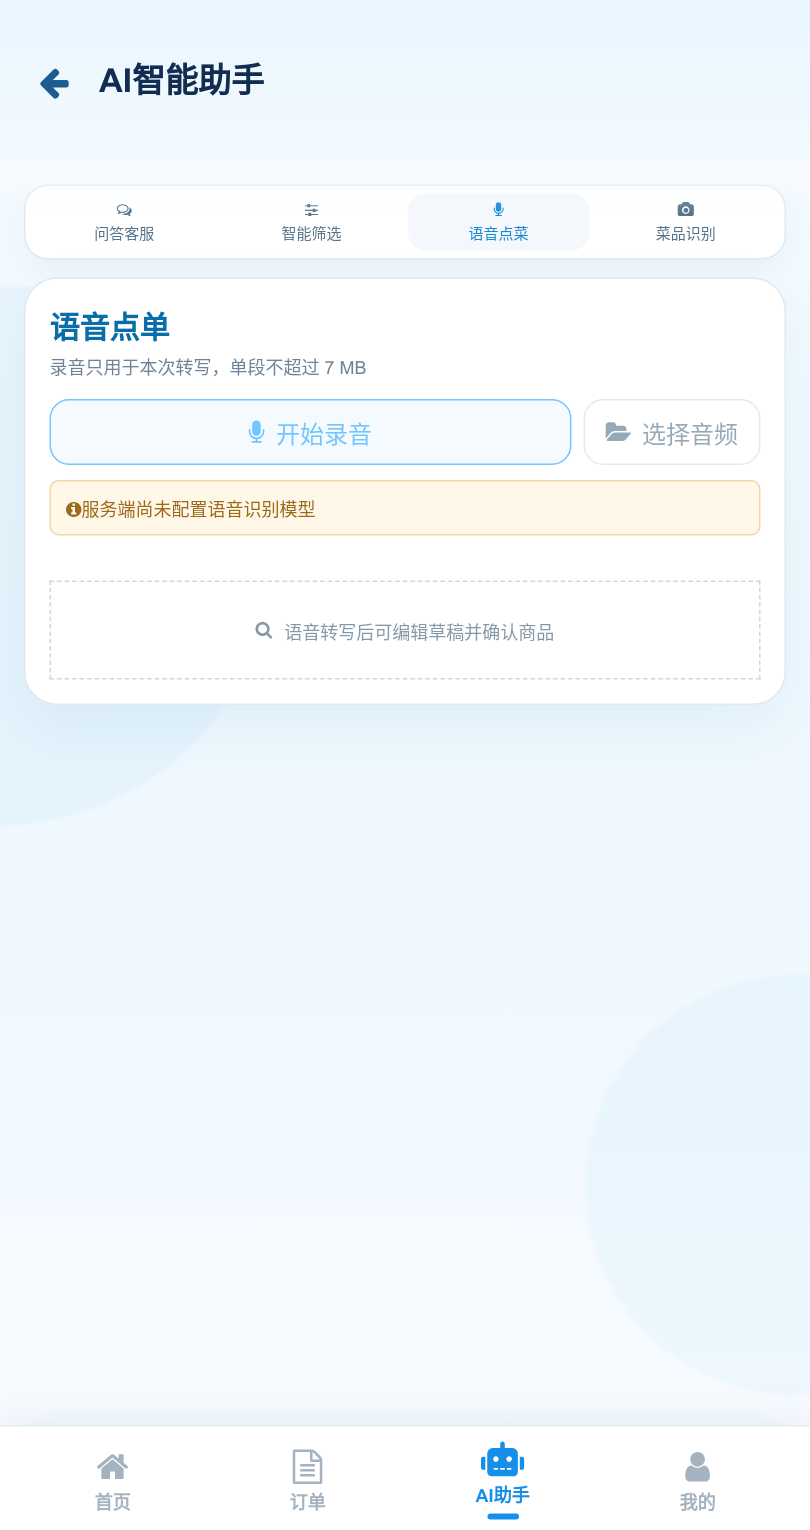
\includegraphics[width=\linewidth,height=.44\textheight,keepaspectratio]{figures/screenshots/ui-ai-voice.png}\par\smallskip
    {\small （a）AI 语音点菜入口与浏览器权限控制（\code{/ai-chat/voice}）}
  \end{minipage}\hfill
  \begin{minipage}[t]{.48\linewidth}
    \vspace{0pt}\centering
    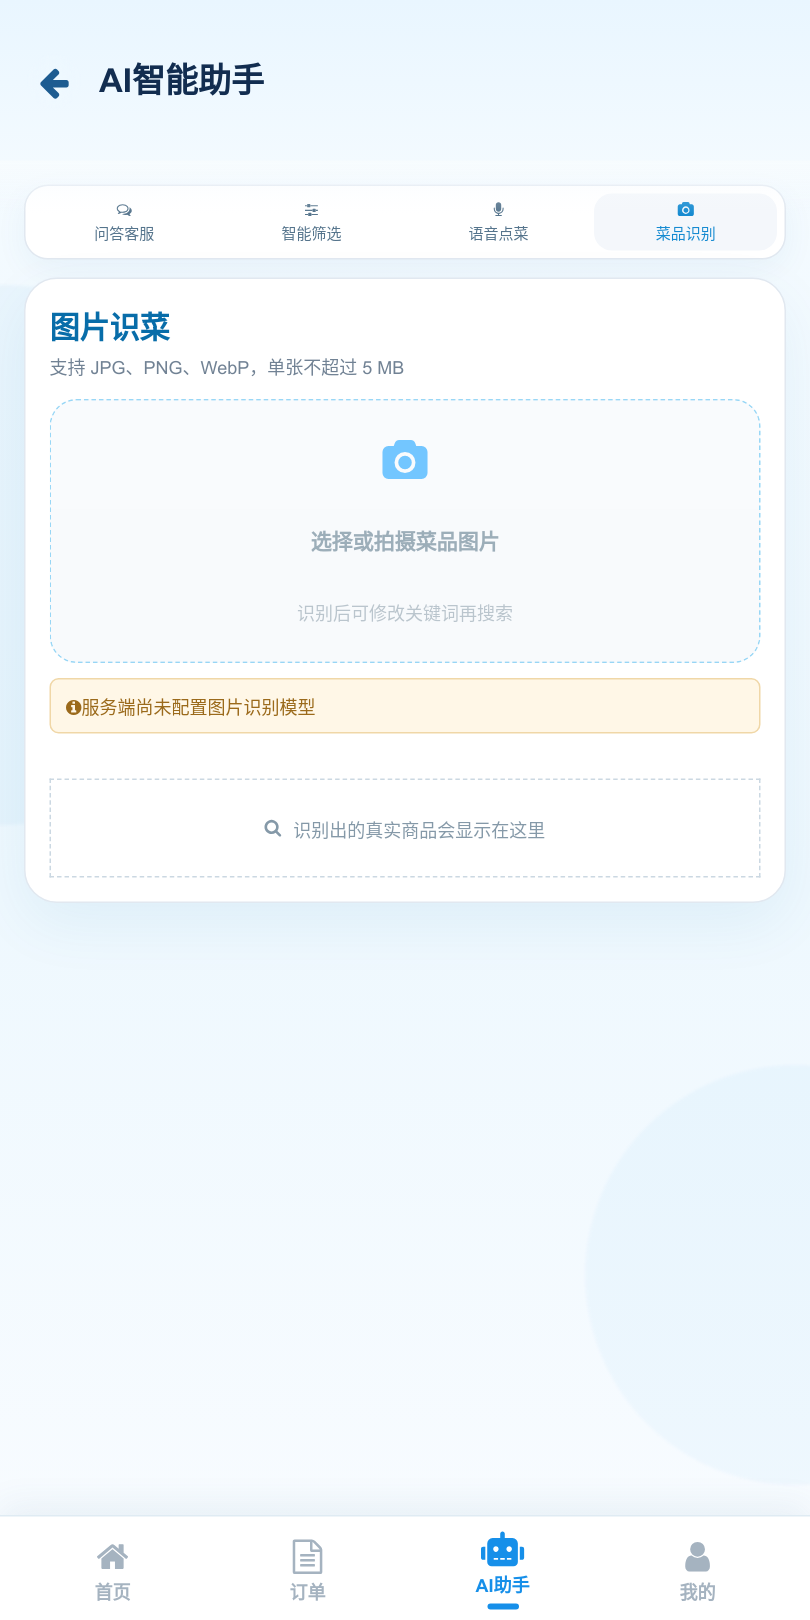
\includegraphics[width=\linewidth,height=.44\textheight,keepaspectratio]{figures/screenshots/ui-ai-media-unconfigured.png}\par\smallskip
    {\small （b）图片识菜模型未配置时的禁用与提示（\code{/ai-chat/image}）}
  \end{minipage}
  \caption{AI 语音点菜与图片识菜未配置降级界面实景截图}\label{fig:ai-voice-media}\label{fig:ai-media-unconfigured}
\end{figure}

接通服务后，语音可以走浏览器授权录音，也可以选本地音频文件。转写出的菜名、份数和预算先放进草稿，顾客改过以后可以重新匹配。图片识菜取出关键词，再列出菜单里的候选。确认具体菜品后，顾客才把它加进购物车。后续验收会从这些动作和页面变化分别检查。

\clearpage
\section{AI 赋能成效评估与核查反思}

\subsection{工程成效评估}

我们用 AI 辅助准备代码样板、SQL 迁移草稿和回归用例。最后交付的是 33 个页面、23 张表和 135 个映射端点，575 项自动化测试均通过。对照历史与现有实现时，我们还找到了 8 项差异，包括订单阶段的叫法和计价顺序。需要继续处理的几项留在表~\ref{tab:gap-improvement}，以后改到相关模块可以回来看。

演示时，顾客在缺少外部模型配置的环境里仍能用本地菜单筛选商品。图片与语音入口依实际状态给出提示，顾客也能返回普通点餐。这是本次走查确认的结果，截图与回归用例分别留住了页面状态和业务判断。

我们在 \code{AssistantIntegrationTest} 里预置了营业和休息的店铺，也给菜品设了不同库存。推荐只返回营业店铺有库存的那一项，对话历史新增一条记录，购物车没有写入。独立推荐接口用同一个预算查两份菜，得到的是空列表。本地退款问答则在历史中标为 \code{local}，模拟历史写入失败后，接口返回服务器错误。这些结果既能从页面找到候选的菜，也能从会话追到产生回复的分支。

\subsection{核查暴露的问题与改进方向}

以后再审阅 AI 草稿，我们会先从一次具体的请求开始。以结算为例，先确认是谁下的单，再看服务端取哪一份价格、最后写下哪些数据。课上讲到，工程师要对交付的结果负责。草稿由谁写并不会改变评审所需的依据，这些字段和断言要由负责该模块的组员核准。

接入有效凭证后，我们计划补测 DeepSeek 对话、DashScope 图片识别和语音转写，记录不同输入的完成率与响应时间。并发时再看单用户 Token 预算、路由调用次数与熔断状态，检查异常请求有没有拖慢普通点餐。未配置画面和超时用例都已留存，可以作为复测的起点。

补测时可以用原来那组菜品、预算与份数。先把能力接口和按钮状态对齐，再逐个试文字、图片与音频，观察识别文本、草稿和候选商品。语音草稿修改份数后再匹配，图片候选可返回具体的店铺菜单。每轮记明服务配置、输入样本与返回状态，耗时按识别、模型生成和菜单匹配分别记录。哪一步失败了，就从该处查起，再确认本地筛选能否继续用。
